% Options for packages loaded elsewhere
\PassOptionsToPackage{unicode}{hyperref}
\PassOptionsToPackage{hyphens}{url}
\PassOptionsToPackage{dvipsnames,svgnames,x11names}{xcolor}
\documentclass[
  10pt,
  fontset=fandol]{ctexart}
\usepackage{xcolor}
\usepackage[margin=16mm]{geometry}
\usepackage{amsmath,amssymb}
\setcounter{secnumdepth}{-\maxdimen} % remove section numbering
\usepackage{iftex}
\ifPDFTeX
  \usepackage[T1]{fontenc}
  \usepackage[utf8]{inputenc}
  \usepackage{textcomp} % provide euro and other symbols
\else % if luatex or xetex
  \usepackage{unicode-math} % this also loads fontspec
  \defaultfontfeatures{Scale=MatchLowercase}
  \defaultfontfeatures[\rmfamily]{Ligatures=TeX,Scale=1}
\fi
\usepackage{lmodern}
\ifPDFTeX\else
  % xetex/luatex font selection
\fi
% Use upquote if available, for straight quotes in verbatim environments
\IfFileExists{upquote.sty}{\usepackage{upquote}}{}
\IfFileExists{microtype.sty}{% use microtype if available
  \usepackage[]{microtype}
  \UseMicrotypeSet[protrusion]{basicmath} % disable protrusion for tt fonts
}{}
\makeatletter
\@ifundefined{KOMAClassName}{% if non-KOMA class
  \IfFileExists{parskip.sty}{%
    \usepackage{parskip}
  }{% else
    \setlength{\parindent}{0pt}
    \setlength{\parskip}{6pt plus 2pt minus 1pt}}
}{% if KOMA class
  \KOMAoptions{parskip=half}}
\makeatother
\usepackage{longtable,booktabs,array}
\newcounter{none} % for unnumbered tables
\usepackage{calc} % for calculating minipage widths
% Correct order of tables after \paragraph or \subparagraph
\usepackage{etoolbox}
\makeatletter
\patchcmd\longtable{\par}{\if@noskipsec\mbox{}\fi\par}{}{}
\makeatother
% Allow footnotes in longtable head/foot
\IfFileExists{footnotehyper.sty}{\usepackage{footnotehyper}}{\usepackage{footnote}}
\makesavenoteenv{longtable}
\usepackage{graphicx}
\makeatletter
\newsavebox\pandoc@box
\newcommand*\pandocbounded[1]{% scales image to fit in text height/width
  \sbox\pandoc@box{#1}%
  \Gscale@div\@tempa{\textheight}{\dimexpr\ht\pandoc@box+\dp\pandoc@box\relax}%
  \Gscale@div\@tempb{\linewidth}{\wd\pandoc@box}%
  \ifdim\@tempb\p@<\@tempa\p@\let\@tempa\@tempb\fi% select the smaller of both
  \ifdim\@tempa\p@<\p@\scalebox{\@tempa}{\usebox\pandoc@box}%
  \else\usebox{\pandoc@box}%
  \fi%
}
% Set default figure placement to htbp
\def\fps@figure{htbp}
\makeatother
\setlength{\emergencystretch}{3em} % prevent overfull lines
\providecommand{\tightlist}{%
  \setlength{\itemsep}{0pt}\setlength{\parskip}{0pt}}
\usepackage{amsmath,amssymb,mathtools,needspace}
\xeCJKDeclareCharClass{CJK}{"2032,"0400->"04FF,"2160->"216B,"2460->"2473,"25A0,"25C7,"25CB,"25CF}
\IfFontExistsTF{Arial Unicode MS}{\xeCJKsetup{AutoFallBack=true}\setCJKfallbackfamilyfont{\CJKrmdefault}{Arial Unicode MS}}{}
\setcounter{secnumdepth}{0}
\setlength{\emergencystretch}{2em}
\allowdisplaybreaks
\usepackage{bookmark}
\IfFileExists{xurl.sty}{\usepackage{xurl}}{} % add URL line breaks if available
\urlstyle{same}
\hypersetup{
  pdftitle={倍增技术},
  colorlinks=true,
  linkcolor={Maroon},
  filecolor={Maroon},
  citecolor={Blue},
  urlcolor={Blue},
  pdfcreator={LaTeX via pandoc}}

\title{倍增技术}
\author{}
\date{}

\begin{document}
\maketitle

\subsubsection{11.2.1　倍增技术}\label{ux500dux589eux6280ux672f}

有些学者认为，倍增技术是设计同步并行算法的一项基本技术。这项设计技术反

\href{../../source-images/pdf-279.jpeg}{原页图像}

复地将计算问题分裂成具有同等规模的两个子问题。在问题逐步分裂的过程中，子问题的个数是逐步倍增的，倍增法因此而得名。

倍增法的设计基于这样的考虑，如果将各个子问题适当地映射到多台处理机上，即可实现计算过程的并行化。

现在就用简单的数列求和问题（11.2.1）考察倍增技术的设计原理和设计方法。为此，引进和式

\[
S(i,j)=\sum_{k=j}^{i}a_k.
\]

显然，问题（11.2.1）的已给数据与所求结果均可用这种和式来表达：

\[
\begin{gathered}
a_i=S(i,i),\quad i=0,1,\cdots,N-1;\\
S=S(N-1,0).
\end{gathered}
\]

倍增法的设计过程含分裂与合成两个环节。分裂过程将所给和式 \(S(N-1,0)\) 逐步``一分为二''，从而拆成若干个子和式。这种分裂过程的特点是，子和式的个数是逐步倍增的。

\[
\begin{aligned}
S(N-1,0)
&=S\left(N-1,\frac{N}{2}\right)+S\left(\frac{N}{2}-1,0\right)\\
&=S\left(N-1,\frac{3}{4}N\right)+S\left(\frac{3}{4}N-1,\frac{N}{2}\right)+S\left(\frac{N}{2}-1,\frac{N}{4}\right)+S\left(\frac{N}{4}-1,0\right)\\
&=\cdots.
\end{aligned}
\]

由于在和式二分的上述过程中，每个子和式的项数逐次减半，因而最终可拆成每段仅含两项的最简形式

\[
S(N-1,0)=S(N-1,N-2)+S(N-3,N-4)+\cdots+S(1,0).
\]

图 11.1 取 \(N=8\) 自顶向下地描述了倍增法的分裂过程。

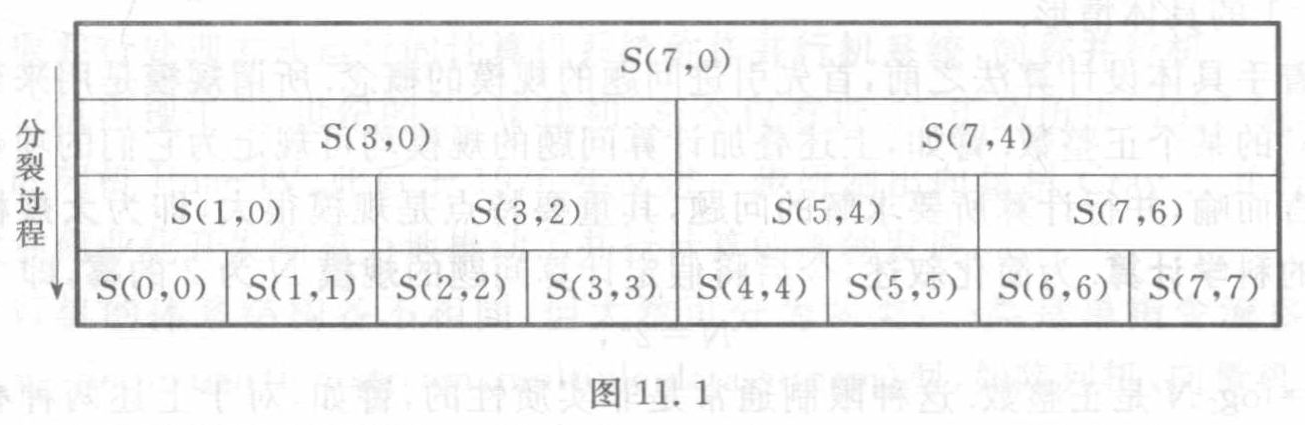
\includegraphics[width=0.85\linewidth,height=\textheight,keepaspectratio,alt={图 11.1（原图裁切）}]{../assets/ch11/figure-11-1.png}

图 11.1　原图的``分裂过程''箭头自上向下。各层由左至右的符号标签为：

{\def\LTcaptype{none} % do not increment counter
\begin{longtable}[]{@{}
  >{\raggedright\arraybackslash}p{(\linewidth - 2\tabcolsep) * \real{0.5000}}
  >{\raggedright\arraybackslash}p{(\linewidth - 2\tabcolsep) * \real{0.5000}}@{}}
\toprule\noalign{}
\begin{minipage}[b]{\linewidth}\raggedright
层次（由上至下）
\end{minipage} & \begin{minipage}[b]{\linewidth}\raggedright
原图中的子和式
\end{minipage} \\
\midrule\noalign{}
\endhead
\bottomrule\noalign{}
\endlastfoot
1 & \(S(7,0)\) \\
2 & \(S(3,0)\)，\(S(7,4)\) \\
3 & \(S(1,0)\)，\(S(3,2)\)，\(S(5,4)\)，\(S(7,6)\) \\
4 & \(S(0,0)\)，\(S(1,1)\)，\(S(2,2)\)，\(S(3,3)\)，\(S(4,4)\)，\(S(5,5)\)，\(S(6,6)\)，\(S(7,7)\) \\
\end{longtable}
}

每个上层区间对应下层相邻的两个子区间。（本段及上表为原图标签与结构的文字转录。）

将所给和式拆成若干个子和式后，可将这些子和式分配给各台处理机去并行计算。问题在于，基于这些子和式的计算，如何得出所求的结果呢？

倍增法的合成过程是将所拆出的各个子和式的值再逐步``合二为一''，最后归并出所给和式的值。这种归并过程的特点是数据量逐次减半。图 11.2 自底向上地描述了倍增法的合成过程。

\href{../../source-images/pdf-280.jpeg}{原页图像}

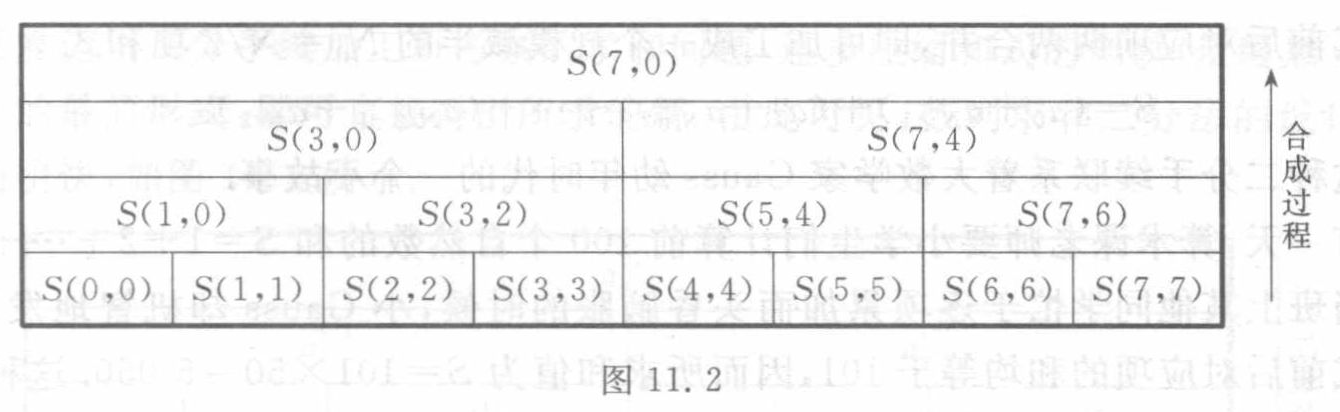
\includegraphics[width=0.85\linewidth,height=\textheight,keepaspectratio,alt={图 11.2（原图裁切）}]{../assets/ch11/figure-11-2.png}

图 11.2　原图``合成过程''箭头自下向上。各层从左至右的符号标签为：

{\def\LTcaptype{none} % do not increment counter
\begin{longtable}[]{@{}
  >{\raggedright\arraybackslash}p{(\linewidth - 2\tabcolsep) * \real{0.5000}}
  >{\raggedright\arraybackslash}p{(\linewidth - 2\tabcolsep) * \real{0.5000}}@{}}
\toprule\noalign{}
\begin{minipage}[b]{\linewidth}\raggedright
层次（由上至下）
\end{minipage} & \begin{minipage}[b]{\linewidth}\raggedright
原图中的子和式
\end{minipage} \\
\midrule\noalign{}
\endhead
\bottomrule\noalign{}
\endlastfoot
1 & \(S(7,0)\) \\
2 & \(S(3,0)\)，\(S(7,4)\) \\
3 & \(S(1,0)\)，\(S(3,2)\)，\(S(5,4)\)，\(S(7,6)\) \\
4 & \(S(0,0)\)，\(S(1,1)\)，\(S(2,2)\)，\(S(3,3)\)，\(S(4,4)\)，\(S(5,5)\)，\(S(6,6)\)，\(S(7,7)\) \\
\end{longtable}
}

每层中相邻的两个子区间向上合成为一个区间。（本段及上表为原图标签与结构的文字转录。）

现在列出倍增法的算法步骤（图 11.2）。

倍增法的第 1 步是利用所给的 \(N\) 个数据（它们均可视为一项和式）\(a_i=S(i,i)\) 求出 2 项和式的值，而得出 \(N_1=N/2\) 个中间结果：

\[
S(2i+1,2i)=S(2i+1,2i+1)+S(2i,2i),\quad i=0,1,\cdots,N_1-1.
\]

第 2 步再用两项和式求出 4 项和式的值，而有 \(N_2=N/4\) 个中间结果：

\[
S(4i+3,4i)=S(4i+3,4i+2)+S(4i+1,4i),\quad i=0,1,\cdots,N_2-1.
\]

保持和式项数逐步倍增，而数据量则为逐次减半这个特征，其第 \(k\) 步所承担的工作是，用 \(2^{k-1}\) 项和式求出 \(2^k\) 项和式的值，从而得出 \(N_k=N/2^k\) 个中间结果：

\[
\begin{gathered}
S(2^ki+2^k-1,2^ki)=S(2^ki+2^k-1,2^ki+2^{k-1})+S(2^ki+2^{k-1}-1,2^ki),\\
i=0,1,\cdots,N_k-1.
\end{gathered}
\tag{11.2.3}
\]

如此做 \(n=\log_2 N\) 步即可得出所求的和值：

\[
S(N-1,0)=S(N-1,N_1)+S(N_1-1,0).
\]

综上所述，数列求和（11.2.1）的倍增法可表述为算法 11.1。

\textbf{算法 11.1}　对 \(k=1,2,\cdots\) 直到 \(n=\log_2 N\) 执行算式（11.2.3），则所求的和值为 \(S=S(N-1,0)\)。

倍增法的分裂过程是反复将和式一分为二，在这一过程中，子和式的个数是逐步倍增的；与此相反，其合成过程是反复将数据合二为一，在合成过程中，数据量则为逐次减半。正是由于倍增法的分裂过程与合成过程相对峙，这种技术不便于实际运用。

\end{document}
